\chapter{From Discrete Observables to Interference}

This chapter follows Leonard Susskind's fourth lecture in the quantum mechanics sequence, and it keeps the blackboard order intact: first the discrete case, then the passage to continuous variables, then the Dirac delta, the particle on a line, the particle on a circle, the incompatibility of position and momentum, and finally the two-slit experiment. It is written as a set of companion notes to the lecture, with explicit credit to Leonard Susskind and with curation support acknowledged to LazyingArt LLC and Video2Book. The main theme is simple to state and worth stating plainly at the outset: the postulates do not change when we move from discrete observables to continuous ones, but the mathematical objects that carry those postulates must be replaced.

\section{Review: Discrete Observables, Probabilities, and Basis States}

Let us begin exactly where the lecture begins: with a measurable quantity that can take discrete values. Call those values \(n=1,2,3,\dots\). If the system is prepared in some state \(|\psi\rangle\), then a measurement of that observable returns one of these values with probability \(P(n)\), and the first rule is the normalization condition
\begin{equation}
\sum_n P(n)=1.
\end{equation}
The second rule is the orthonormality of the basis states \(|n\rangle\):
\begin{equation}
\langle m|n\rangle=\delta_{nm}.
\end{equation}
Here \(\delta_{nm}\) is the Kronecker delta. It is \(1\) when \(n=m\) and \(0\) otherwise. Susskind pauses over the point that this can be regarded as a function of the difference \(n-m\); the statement of orthogonality depends only on whether that difference vanishes.

The probability itself is governed by amplitudes. In the discrete case the amplitude for finding the value \(n\) is \(\langle n|\psi\rangle\), and the corresponding probability is
\begin{equation}
P(n)=|\langle n|\psi\rangle|^2.
\end{equation}
So the discrete picture contains all the elements we will need later: normalization, orthonormal basis vectors, amplitudes, and a rule for turning amplitudes into probabilities.

\begin{figure}
\centering

\includegraphics[width=0.62\textwidth]{lecture_04_figure_02.png}
\end{figure}

If one plots the probability as a function of a discrete variable, the values live only at the integers. The picture is therefore not a continuous curve but a collection of heights, one above each allowed value of \(n\), and it is those heights that add up to \(1\).

\begin{figure}
\centering
\begin{tikzpicture}[x=1.3cm,y=1.1cm]
\draw[->] (0,0) -- (4.8,0) node[right] {$n$};
\draw[->] (0,0) -- (0,2.9) node[above] {$P(n)$};
\foreach \x/\h in {0.9/1.8,1.8/0.9,2.7/1.3,3.6/0.6}
{
  \draw (\x,0) -- (\x,\h);
  \fill (\x,\h) circle (0.05);
}
\node[below] at (0.9,0) {$1$};
\node[below] at (1.8,0) {$2$};
\node[below] at (2.7,0) {$3$};
\node[below] at (3.6,0) {$4$};
\node at (3.2,2.35) {$\sum_n P(n)=1$};
\end{tikzpicture}
\end{figure}

This is not just review for its own sake. It is the template for everything that follows. The lecture is constructed as a sequence of replacements: when the observable ceases to be discrete, sums will be replaced by integrals, and Kronecker deltas by Dirac deltas, but the formal logic remains the same.

\section{From Discrete Probabilities to Continuous Probability Density}

Now let the observable be the position of a particle on a line. The first thing that breaks is not the amplitude story but the ordinary language of probability. It no longer makes sense to ask for the probability that the coordinate is exactly equal to one specific real number. A single point has measure zero, and the probability of one exact value is therefore zero.

What makes sense instead is the probability that the particle lies in an interval. We introduce a probability density, which I will denote by \(P(x)\) in order to keep it visually separate from the later use of \(p\) for momentum. The probability that the particle is found between \(x\) and \(x+\Delta x\) is then
\begin{equation}
P\bigl(x\in [x,x+\Delta x]\bigr)=\int_x^{x+\Delta x} P(x')\,dx'.
\end{equation}
The normalization rule changes accordingly:
\begin{equation}
\int P(x)\,dx = 1.
\end{equation}
This is the continuum version of \(\sum_n P(n)=1\). In the discrete picture the heights themselves add to \(1\); in the continuous picture it is the area under the curve that must be \(1\).

\begin{figure}
\centering

\includegraphics[width=0.68\textwidth]{lecture_04_figure_03.png}
\end{figure}

The lecture uses a bell-shaped curve only as a schematic. Nothing essential depends on that particular shape. The point is simply that a continuous variable is described by a density, and the physically meaningful probability is the area under the density over some interval.

\begin{figure}
\centering
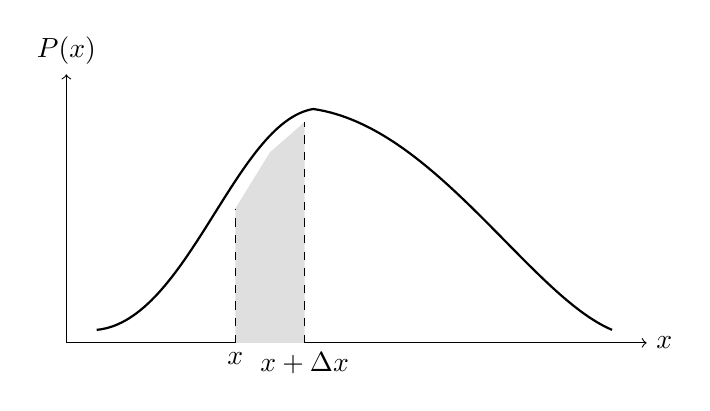
\begin{tikzpicture}[x=1.1cm,y=1.1cm]
\draw[->] (0,0) -- (6.7,0) node[right] {$x$};
\draw[->] (0,0) -- (0,3.1) node[above] {$P(x)$};
\draw[thick]
  (0.35,0.15)
  .. controls (1.4,0.25) and (1.95,2.55) ..
  (2.85,2.7)
  .. controls (4.25,2.5) and (5.35,0.55) ..
  (6.3,0.15);
\fill[gray!25]
  (1.95,0) --
  (1.95,1.55) --
  (2.35,2.2) --
  (2.75,2.55) --
  (2.75,0) -- cycle;
\draw[dashed] (1.95,0) -- (1.95,1.55);
\draw[dashed] (2.75,0) -- (2.75,2.55);
\node[below] at (1.95,0) {$x$};
\node[below] at (2.75,0) {$x+\Delta x$};
\end{tikzpicture}
\end{figure}

At this point the first replacement is complete. But there is a second one waiting. If the basis is now labeled by a continuous variable, what replaces the inner product \(\langle m|n\rangle=\delta_{nm}\)? Before answering that, the lecture quite deliberately stops to discuss the Dirac delta.

\section{The Dirac Delta and Born's Rule on a Line}

The Dirac delta is introduced as the continuous analogue of the Kronecker delta. One first thinks of it heuristically and only then operationally. Heuristically, \(\delta(x-y)\) is zero when \(x\neq y\), sharply peaked at \(x=y\), and normalized so that the total area under the spike is \(1\):
\begin{equation}
\delta(x-y)=0 \quad \text{for } x\neq y,
\qquad
\int \delta(x-y)\,dx=1.
\end{equation}
This is not an honest function in the elementary sense, and Susskind says so. The mathematically serious content is its action under integration:
\begin{equation}
\int \delta(x-y)f(x)\,dx = f(y).
\end{equation}
The logic is simple. Since the delta vanishes everywhere except at \(x=y\), only the value of the function at \(y\) can matter.

With that tool in hand, we can now write the continuum version of orthogonality:
\begin{equation}
\langle x|y\rangle = \delta(x-y).
\end{equation}
The vector space is now the vector space of complex functions of the real variable \(x\), and its inner product is
\begin{equation}
\langle \phi|\psi\rangle = \int \phi^*(x)\psi(x)\,dx.
\end{equation}
A state in which the particle is known to be at \(y\) is represented in the \(x\)-representation by the function \(\delta(x-y)\). Therefore the amplitude to find the particle at \(y\) in the state \(|\psi\rangle\) is
\begin{align}
\langle y|\psi\rangle
  &= \int \delta(x-y)\psi(x)\,dx \\
  &= \psi(y).
\end{align}
This is the continuum Born rule rebuilt from the abstract postulates, not introduced as a separate guess. The wavefunction at \(y\) is the amplitude to detect the particle at \(y\). Therefore the probability density is
\begin{equation}
P(y)=|\langle y|\psi\rangle|^2 = |\psi(y)|^2 = \psi^*(y)\psi(y).
\end{equation}

\subsection{Question \& Answer}

\paragraph{Question.} How can \(\langle x|y\rangle\) be a delta function, and in what sense can a position eigenvector have infinite norm?

\paragraph{Answer.} The lecture answers this by stepping back to a dense discrete approximation. Replace the line by lattice sites separated by a tiny spacing \(a\), and let \(|n\rangle\) be the orthonormal basis with
\[
\langle n|m\rangle=\delta_{nm}.
\]
Now identify the continuum position state with a rescaled lattice state,
\[
|x\rangle = \frac{1}{\sqrt a}\,|n\rangle.
\]
Then
\begin{equation}
\langle x|y\rangle = \frac{1}{a}\,\delta_{nm}.
\end{equation}
That object is zero unless the two sites coincide, and when they do coincide its height is \(1/a\). As \(a\to 0\), this becomes precisely the narrow spike of width \(a\) and height \(1/a\) whose area is \(1\). In this sense the Dirac delta differs from the Kronecker delta by the spacing factor.

So yes: the continuum-normalized position vectors have divergent norm. But this is not a practical problem because we almost never need \(\langle x|x\rangle\) by itself. What we use is the delta function under an integral, where it does exactly the work we want. The infinite norm is the price of choosing a normalization adapted to continuum integration rather than to discrete summation.

\section{Particle on a Circle: Periodicity, Momentum Eigenfunctions, and Quantization}

The next move in the lecture is important: the formalism does not change, but the system does. Instead of a particle on an infinite line, we study a particle moving on a circle of radius \(R\). To make contact with the previous notation, one cuts the circle at some point and lays it out as an interval
\[
0 \le x \le 2\pi R.
\]
The new ingredient is periodicity. A function on the circle must come back to itself after one full turn:
\begin{equation}
\psi(x+2\pi R)=\psi(x).
\end{equation}
This is the essential restriction on the state space. The allowable wavefunctions are the periodic complex functions on the interval. They do form a vector space: multiplying a periodic function by a complex number preserves periodicity, and adding two periodic functions preserves it as well.

Now the lecture returns to momentum. In the \(x\)-representation, the momentum operator acts as
\begin{equation}
\hat p = -i\hbar\,\frac{\partial}{\partial x}.
\end{equation}

\begin{figure}
\centering

\includegraphics[width=0.68\textwidth]{lecture_04_figure_04.png}
\end{figure}

Its eigenvalue equation is
\begin{equation}
-i\hbar\,\frac{\partial}{\partial x}\psi(x)=p\,\psi(x).
\end{equation}
Solving this first-order differential equation is immediate:
\begin{align}
\frac{\partial \psi}{\partial x} &= \frac{ip}{\hbar}\,\psi, \\
\psi_p(x) &= C\,e^{ipx/\hbar}.
\end{align}
So the momentum eigenfunctions are plane waves. This is one of the places where the wavefunction earns its name.

The lecture then normalizes these eigenfunctions on the circle.

\begin{figure}
\centering

\includegraphics[width=0.54\textwidth]{lecture_04_figure_05.png}
\end{figure}

The frame shows the integral \(\int \psi^*\psi\,dx\) being written; the equality to \(1\) comes from the transcript. On the circle the normalization condition is
\begin{equation}
\int_0^{2\pi R}\psi_p^*(x)\psi_p(x)\,dx = 1.
\end{equation}
Since \(\psi_p(x)=C e^{ipx/\hbar}\), we have \(\psi_p^*\psi_p=|C|^2\), and therefore
\begin{equation}
1 = |C|^2 \int_0^{2\pi R} dx = 2\pi R\,|C|^2.
\end{equation}
Thus
\begin{equation}
C=\frac{1}{\sqrt{2\pi R}}
\end{equation}
up to an irrelevant phase, and the normalized eigenfunction is
\begin{equation}
\psi_p(x)=\frac{1}{\sqrt{2\pi R}}\,e^{ipx/\hbar}.
\end{equation}

\begin{figure}
\centering

\includegraphics[width=0.75\textwidth]{lecture_04_figure_06.png}
\end{figure}

The last frame is partly occluded, so the exact chalk label on the bra-ket side is not perfectly secure, but the transcript settles the intended relation:
\begin{equation}
\langle x|p\rangle = \frac{1}{\sqrt{2\pi R}}\,e^{ipx/\hbar}.
\end{equation}
That is, a momentum eigenvector, when represented in the position basis, is a normalized plane wave.

Now comes the real payoff. Not every plane wave is allowed, because not every plane wave is periodic. We must impose
\begin{equation}
e^{ip(x+2\pi R)/\hbar}=e^{ipx/\hbar}.
\end{equation}
Cancelling the common factor \(e^{ipx/\hbar}\), we obtain
\begin{equation}
e^{i2\pi Rp/\hbar}=1.
\end{equation}
This holds precisely when the exponent is an integer multiple of \(2\pi i\):
\begin{equation}
\frac{2\pi Rp}{\hbar}=2\pi n,
\qquad n\in \mathbb{Z}.
\end{equation}
Therefore the allowed momenta are quantized:
\begin{equation}
p_n=\frac{n\hbar}{R}.
\end{equation}
The position on the circle is continuous, but the momentum is discrete. This is the origin of quantization in the lecture: periodicity of the wavefunction.

If we now define the angular momentum in the classical way,
\begin{equation}
L=Rp,
\end{equation}
then the allowed angular momenta are
\begin{equation}
L_n=Rp_n=n\hbar.
\end{equation}
The factor of \(R\) cancels. This is why angular momentum is quantized in units of \(\hbar\), independent of the radius of the circle.

\subsection{Question \& Answer}

\paragraph{Question.} Does the large-\(R\) limit give us classical mechanics, or only a dense momentum spectrum?

\paragraph{Answer.} Only a dense spectrum. As \(R\to\infty\), the spacing between adjacent allowed momenta,
\[
\Delta p = \frac{\hbar}{R},
\]
goes to zero. The discrete spectrum becomes dense, and the lecture says that in this limit it is convenient to pass from Kronecker-delta normalization to Dirac-delta normalization in momentum space. But this does not yet recover classical mechanics.

Classical mechanics would require something stronger: states with simultaneously definite position and definite momentum. The large-\(R\) limit does not provide that. It only tells us that the momentum eigenvalues become closely packed. The real obstruction to classical simultaneity lies elsewhere, namely in the incompatibility of the position and momentum operators. That is the next subject.

\section{Compatibility, Common Eigenvectors, and the Commutator \texorpdfstring{\([x,p]\)}{[x,p]}}

The lecture now pivots from spectra to states. Classical mechanics allows a particle to have a sharp position and a sharp momentum at the same time. Quantum mechanics does not. The reason is not that momentum on the line is continuous and momentum on the circle is discrete. The real issue is compatibility.

Suppose we have two observables represented by operators \(A\) and \(B\). They are compatible if there exists a complete basis of vectors that are eigenvectors of both operators at once. Write
\begin{equation}
A|n\rangle = \alpha_n |n\rangle,
\qquad
B|n\rangle = \beta_n |n\rangle.
\end{equation}
Then, on that common eigenbasis,
\begin{equation}
AB|n\rangle = \alpha_n \beta_n |n\rangle
\end{equation}
and also
\begin{equation}
BA|n\rangle = \beta_n \alpha_n |n\rangle.
\end{equation}
Since ordinary numbers commute, these are the same. This motivates the criterion
\begin{equation}
[A,B]\equiv AB-BA=0.
\end{equation}
The lecture states that this condition is not merely necessary but also sufficient: two observables are compatible precisely when their commutator vanishes.

Position and momentum do not satisfy this condition. The position eigenstates are sharply localized delta functions; the momentum eigenstates are plane waves, spread out over all space. They do not share eigenvectors. Susskind then computes the commutator explicitly.

Let \(x\) act by multiplication and let \(p\) act as \(-i\hbar\,\partial_x\). To determine the operator \(xp-px\), apply it to an arbitrary wavefunction \(\psi(x)\):
\begin{align}
(xp-px)\psi(x)
  &= x\!\left(-i\hbar\,\frac{d\psi}{dx}\right)
     -\left(-i\hbar\,\frac{d}{dx}\right)\!\bigl(x\psi(x)\bigr) \\
  &= -i\hbar\,x\frac{d\psi}{dx}
     + i\hbar\,\frac{d}{dx}\bigl(x\psi(x)\bigr).
\end{align}
Now use the product rule:
\begin{equation}
\frac{d}{dx}\bigl(x\psi(x)\bigr)=\psi(x)+x\frac{d\psi}{dx}.
\end{equation}
Substituting,
\begin{align}
(xp-px)\psi(x)
  &= -i\hbar\,x\frac{d\psi}{dx}
     + i\hbar\left(\psi(x)+x\frac{d\psi}{dx}\right) \\
  &= i\hbar\,\psi(x).
\end{align}
Since this holds for every \(\psi(x)\), the operator identity is
\begin{equation}
[x,p]=xp-px=i\hbar.
\end{equation}

This is the formal hinge of the lecture. As a statement about ordinary numbers it would be nonsense, since \(xp=px\). But \(x\) and \(p\) here are operators, and operators need not commute. In fact, Susskind emphasizes that this is about as strong a failure of commutativity as one can have: the commutator is not another complicated operator but a pure number. That is why there are no common eigenvectors at all.

\section{Two-Slit Interference as Superposition of States}

The lecture now cashes out the formalism in the two-slit experiment. The main point is not geometric optics. It is superposition. Quantum states can be added, and probabilities are computed only after squaring the resulting amplitude.

Start with one slit open. The wave emerging from one hole spreads out and reaches the screen with a varying phase. Globally it is not exactly a pure plane wave in the vertical coordinate \(y\), but over a small interval it can be approximated that way. More faithfully, the lecture describes the one-hole wavefunction heuristically as
\begin{equation}
\psi_{\text{1-hole}}(y)\sim e^{i\varphi(y)}\rho(y),
\end{equation}
where \(\rho(y)\) is a slowly varying envelope and \(\varphi(y)\) is a rapidly varying phase. An alternative heuristic form, also given in the lecture, is the outgoing spherical-wave expression
\begin{equation}
\psi(r)\sim \frac{e^{ipr}}{r},
\qquad
r=\sqrt{\ell^2+y^2}.
\end{equation}
The point of writing it this way is that the phase is \(pr\), not simply \(py\), so the local vertical oscillation rate changes with \(y\). The farther one goes from the center, the larger the vertical momentum component that must have been picked up, and the faster the oscillation becomes.

\subsection{Question \& Answer}

\paragraph{Question.} Why does one hole give a smooth blob, while two holes can create dark fringes where no particle ever lands?

\paragraph{Answer.} For one hole, the phase oscillates but the probability is obtained by multiplying the wavefunction by its complex conjugate:
\begin{equation}
|\psi_{\text{1-hole}}(y)|^2
  \sim \bigl(e^{i\varphi(y)}\rho(y)\bigr)\bigl(e^{-i\varphi(y)}\rho(y)\bigr)
  = \rho(y)^2.
\end{equation}
The phase cancels. What remains is the smooth envelope. So the probability from one hole may form a broad blob, but the rapid oscillation of the amplitude does not by itself generate visible oscillation in the probability.

With two holes open, however, the total state is not one amplitude or the other. It is the sum of amplitudes:
\[
\psi=\psi_1+\psi_2.
\]
When we square that sum, cross-terms survive, and those cross-terms carry the relative phase. That is exactly where the interference pattern comes from.

To see the algebra cleanly, let us work locally on the screen and use units in which \(\hbar=1\). Approximate the two contributions by
\begin{equation}
\psi_1(y)\approx e^{ipy},
\qquad
\psi_2(y)\approx e^{iqy}.
\end{equation}
Each one separately has constant magnitude, so each one separately would give a uniform probability over that small interval. But with both holes open,
\begin{align}
|\psi_1+\psi_2|^2
  &= (e^{ipy}+e^{iqy})(e^{-ipy}+e^{-iqy}) \\
  &= 1+1+e^{i(p-q)y}+e^{i(q-p)y} \\
  &= 2+2\cos\bigl((p-q)y\bigr).
\end{align}
This is not constant. It oscillates. In particular, there are values of \(y\) for which the cosine is \(-1\), and then the probability is zero. These are the dark fringes.

This is the core phenomenon. Open slit \(1\) alone and the particle can arrive at a given point. Open slit \(2\) alone and the particle can arrive there as well. Open both together and there are points that never register a hit in the idealized limit. The puzzle is not that waves interfere. The puzzle is that the interference pattern persists even when one sends particles through one at a time. The accumulated spots on the screen build up the same distribution. The probability is always nonnegative, because it is obtained from an amplitude times its complex conjugate, but it can vanish exactly in the ideal limit.

The spacing of the fringes follows the lecture's beat pattern as well. If the two slits are very close together, then the local vertical frequencies \(p\) and \(q\) are almost the same, so \(p-q\) is small and the cosine varies slowly. The fringe spacing is large. If the slits are farther apart, then \(p\) and \(q\) differ more, and the fringes become more closely spaced.

The lecture stops at exactly the right place. It does not yet explain what happens when a detector is placed at a slit to determine which path the particle took. That question belongs to composite systems, to the tensor-product structure of the state space, and to entanglement. The same is true of the question of reversing the motion after the particle has been recorded on a screen. Those are deferred until Hamiltonians and time evolution have been introduced.

\section{Summary}

The arc of the lecture is now visible as one continuous mathematical story. We began with a discrete observable, with probabilities \(P(n)\), orthonormal basis vectors, and the Kronecker delta. We then replaced exact point-probabilities by interval probabilities, sums by integrals, and the Kronecker delta by the Dirac delta. That allowed us to rebuild the continuum Born rule on the line in the form \(P(y)=\psi^*(y)\psi(y)\). Moving from the line to the circle changed not the formalism but the allowed state space: periodicity of the wavefunction forced momentum and angular momentum to become quantized. From there the lecture turned to the deeper issue of compatibility, culminating in the operator identity
\[
[x,p]=i\hbar,
\]
which expresses the failure of position and momentum to be simultaneously sharp. The two-slit experiment then served as the physical payoff: amplitudes add, probabilities do not, and the cross-term in \(|\psi_1+\psi_2|^2\) produces the interference pattern, including dark fringes where no particles arrive.